\section{Problem}

The Medical test Records project approaches two main problems that hospital information systems must face. \\

The first originates from the sensible information that must be stored in order for the doctors, nurses, assistants... be able to give patients the necessary treatment. A patient profile has associated to it a group of information with different levels of sensibility for example: age, name, blood type, diseases, family records... 
A name is not something sensible so probably most employees can access it, but what about the patient family records? A volunteer has no need to know such information. \\

Given this scenario, the information systems in cause must be able to provide and enforce the correct policies so that different parts of a patient profile are only available to who actually need it and in the correct context. \\

The second problem is in the way that medical tests must be analyzed in different facilities, like partner labs, that are not part of the hospital infrastructure, but require that both are interconnected in a way that enables all sides to identify each other and communicate in a safe and secure way. \\

\subsection{Requisites}

Given the previous problems, the implementation of this project requires the following security guarantees:
\begin{itemize}
	\item A fine grained access control.
	\item Integrity of all communications with the information systems.
	\item Confidentiality of all communications with the information systems.
	\item Non-repudiation of the tests results data.
	\item Authenticity of the tests results data.
\end{itemize}

\subsection{Trust assumptions}

The main entities in this project are two, the hospital information system and the clients that try to access said system. \\

The client entity can be internal or external to the hospital infrastructure, if the context is internal, the client is used by the hospital staff (doctors, nurses...). In case the client is used by the partner labs to send the tests data result, the client is external. \\

In both cases the client is untrusted, the information systems will require some type of authentication and authorization before the request is accepted. \\ 

There is also a full trust assumption, that the code responsible for the access control is error free and an unauthorized person will never be able to access something is not supposed. \\

\section{Solução Proposta}

The implementation will be separated in two main components, a REST API and a client of the API.
The API will 

	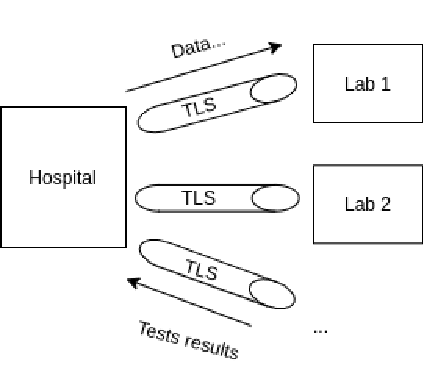
\includegraphics{figs/server_client.pdf}
	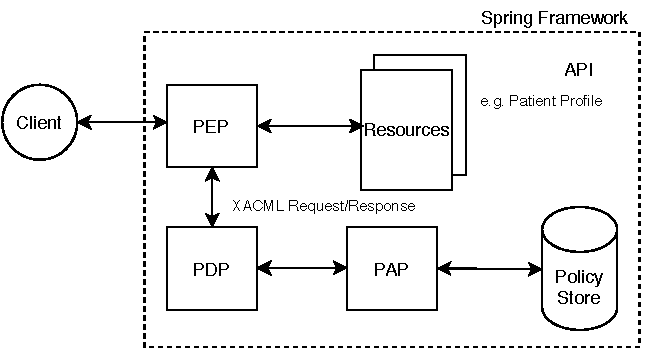
\includegraphics{figs/access_control.pdf}
	

\section{Plano}

\section{Referências}